\documentclass[unicode,11pt,a4paper,oneside,numbers=endperiod,openany]{scrartcl}

\renewcommand{\thesubsection}{\arabic{subsection}}

\usepackage{ifthen}
\usepackage[utf8]{inputenc}
\usepackage{graphics}
\usepackage{graphicx}
\usepackage{hyperref}

\pagestyle{plain}
\voffset -5mm
\oddsidemargin  0mm
\evensidemargin -11mm
\marginparwidth 2cm
\marginparsep 0pt
\topmargin 0mm
\headheight 0pt
\headsep 0pt
\topskip 0pt        
\textheight 255mm
\textwidth 165mm

\newcommand{\duedate} {}
\newcommand{\setduedate}[1]{%
\renewcommand\duedate {\textbf{Due date:}~ #1}}
\newcommand\isassignment {false}
\newcommand{\setassignment}{\renewcommand\isassignment {true}}
\newcommand{\ifassignment}[1]{\ifthenelse{\boolean{\isassignment}}{#1}{}}
\newcommand{\ifnotassignment}[1]{\ifthenelse{\boolean{\isassignment}}{}{#1}}

\newcommand{\assignmentpolicy}{
\begin{table}[h]
\begin{center}
\scalebox{0.8} {%
\begin{tabular}{|p{0.02cm}p{16cm}|}
\hline
&\\
\multicolumn{2}{|c|}{\Large\textbf{Numerical Computing 2023 ---  Submission Instructions}}\\
\multicolumn{2}{|c|}{\large\textbf{(Please, notice that following instructions are mandatory: }}\\
\multicolumn{2}{|c|}{\large\textbf{submissions that don't comply with, won't be considered)}}\\
&\\
\textbullet & Assignments must be submitted to \href{https://www.icorsi.ch/course/view.php?id=14666}{iCorsi} (i.e. in electronic format).\\
\textbullet & Provide both executable package and sources (e.g. C/C++ files, MATLAB). 
If you are using libraries, please add them in the file. Sources must be organized in directories called:\\
\multicolumn{2}{|c|}{\textit{Project\_number\_lastname\_firstname}}\\
& and  the  file must be called:\\
\multicolumn{2}{|c|}{\textit{project\_number\_lastname\_firstname.zip}}\\
\multicolumn{2}{|c|}{\textit{project\_number\_lastname\_firstname.pdf}}\\
\textbullet &  The TAs will grade your project by reviewing your project write-up, and looking at the implementation you attempted, and benchmarking your code's performance.\\

\textbullet & You are allowed to discuss all questions with anyone you like; however: (i) your submission must list anyone you discussed problems with and (ii) you must write up your submission independently.\\
\hline
\end{tabular}
}
\end{center}
\end{table}
}
\newcommand{\punkte}[1]{\hspace{1ex}\emph{\mdseries\hfill(#1~\ifcase#1{Points}\or{Points}\else{Points}\fi)}}


\newcommand\serieheader[6]{
\thispagestyle{empty}%
\begin{flushleft}

\includegraphics[width=0.45\textwidth]{CI_logo}
\end{flushleft}
  \noindent%
  {\large\ignorespaces{\textbf{#1}}\hspace{\fill}\ignorespaces{ \textbf{#2}}}\\ \\%
  {\large\ignorespaces #3 \hspace{\fill}\ignorespaces #4}\\
  \noindent%
  \bigskip
  \hrule\par\bigskip\noindent%
  \bigskip {\ignorespaces {\Large{\textbf{#5}}}
  \hspace{\fill}\ignorespaces \large \ifthenelse{\boolean{\isassignment}}{\duedate}{#6}}
  \hrule\par\bigskip\noindent%  \linebreak
 }

\makeatletter
\def\enumerateMod{\ifnum \@enumdepth >3 \@toodeep\else
      \advance\@enumdepth \@ne
      \edef\@enumctr{enum\romannumeral\the\@enumdepth}\list
      {\csname label\@enumctr\endcsname}{\usecounter
        {\@enumctr}%%%? the following differs from "enumerate"
	\topsep0pt%
	\partopsep0pt%
	\itemsep0pt%
	\def\makelabel##1{\hss\llap{##1}}}\fi}
\let\endenumerateMod =\endlist
\makeatother




\usepackage{textcomp}





\usepackage{listings}
\usepackage{xcolor}
\usepackage{float}
\usepackage{amsmath}
\usepackage{amsmath, amssymb} % for math symbols and fonts
\usepackage{hyperref} % for hyperlinks

\definecolor{codegreen}{rgb}{0,0.6,0}
\definecolor{codegray}{rgb}{0.5,0.5,0.5}
\definecolor{codepurple}{rgb}{0.58,0,0.82}
\definecolor{backcolour}{rgb}{0.95,0.95,0.92}

\lstdefinestyle{mystyle}{
    language=Matlab,
    backgroundcolor=\color{backcolour},
    commentstyle=\color{codegreen},
    keywordstyle=\color{blue},
    numberstyle=\tiny\color{codegray},
    numbers=left,
    numbersep=5pt,
    basicstyle=\ttfamily\footnotesize,
    breakatwhitespace=false,
    breaklines=true,
    captionpos=b,
    keepspaces=true,
    showspaces=false,
    showstringspaces=false,
    showtabs=false,
    tabsize=2
}

\lstnewenvironment{mcode}[1][]
{\lstset{style=mystyle,#1}}
{}

\begin{document}


\setassignment
\setduedate{Wednesday, 11 October 2023, 23:59 AM}

\serieheader{Numerical Computing}{2023}{\textbf{Student:} Harkeerat Singh Sawhney}{\textbf{Discussed with:} Guerrero Toro Cindy}{Solution for Project 1}{}
\newline

\assignmentpolicy


\newpage

\subsection{Theoretical questions [15 points]}

\begin{enumerate}
    \item[(a)] \textbf{What are an eigenvector, an eigenvalue and an eigenbasis?} \\
          \textbf{Eigenvector:} In linear transformation an eigenvector is a non-zero vector that can get changed through a constant factor when the linear transformation is applied on it. When the eigenvector is linearly transformed only the scale is changed not the direction. \\

          \textbf{Eigenvalue:} Eigenvalue is often represented with $ \lambda $ which is the multiplying factor which determines how much the eigenvector is linearly transformed along the direction. It is the factor by which the eigenvector is stretched or compressed. \\

          \textbf{Eigenbasis:} Eigenbasis is a diagonal matrix that has eigenvalues along the diagonal and eigenvectors its columns.  Eigenbasis are helpful in cases where functions such as matrix powers, exponentials and other similar functions needs to be performed due to the simplification in the computation.


    \item[(b)] \textbf{What assumptions should be made to guarantee convergence of the power method?}
          Firstly, we need to assume that the randomly chosen initial vectors must be part of the same direction as the eigenvector. We also need to assume that in the eigenvector which is used to get the Page Rank convergence is the dominant eigenvalue. $ \lambda_1$ and $ \lambda_2$ need to be distance to assure a faster convergence. Since the asymptotic error is constant $\frac{\lambda_1}{\lambda_2}$, this means that if the eigenvectors are close to each other then the convergence would be very slow.
    \item[(c)] \textbf{What is the shift and invert approach?}
          In Shift and Invert technique if the eigenvalue of A are $ \lambda_j $ then the eigenvalues of $A - \alpha I $ are $\lambda_j - \alpha$ and the eigenvalues of $ B = (A - \alpha I)^{-1}$ would be as follows:

          $$ \mu_j = \frac{1}{\lambda_j - \alpha} $$

          From this we can see that the close $\alpha$ is to $\lambda_j$ the larger and more dominant the largest eigenvalue of $B$ will be. This would be mean that if the limit $\alpha -> \lambda_1$ then the first eigenvalue of B to would be going to infinity whereas other eigenvalues would be going to finite values.

          Therefoere now if we apply the power method to $ B = (A - \alpha I)^{-1}$ rather than towards A, and we also asume that $ \lambda_2$ is the eigenvalue of A which is the closest to $\lambda_1$. With such iteration we would converge linearly, but the rate of convergence would be much faster than the power method.

    \item[(d)] \textbf{What is the difference in cost of a single iteration of the power method, compared to the inverse iteration?}

          When Power Method is used, in each iteration there would be a matrix-vector multiplication where in the Inverse Iteration we would be solving a linear system. It is computationly expensive to solve a linear system than to perform a matrix-vector multiplication. In order to use the inverse iteration, we must have a fast convergence for the inverse iteration to be faster than the power method. Realisticly speaking this would be very tought to implement in real world scenarios such as the PageRank problem on the web. Hence Inverse Iteration should be used for small problems where the matrix is small and dense.

    \item[(e)] \textbf{What is a Rayleigh quotient and how can it be used for eigenvalue computations?}

          Rayleigh quotient is a form of Inverse Itearation, but the difference is the method in which the eigenvalues are found. Rayleigh quotient guarantees fast convergence, because it change the value of $\alpha$ in each iteration. The value of $\alpha$ is changed in each iteration to the Rayleigh quotient of the current vector. With this approach the convergence speed increases as we get closer to the eigenvalue. With this the convergence speed is better than linear. The convergence speed in fact in most cases is cubic. Hence it is worth paying the price for having to refactor the matrix in every iteration.
\end{enumerate}

\subsection{Connectivity matrix and subcliques [5 points]}
By observing the spy plot, it was observed that there starting from the range 73-100 there were in total 11 cliques. Hence by manually noting down the ranged of the indices for the cliques, the dominant organization was found. Bellow is an example of how the first cliques was found. \\

\begin{mcode}
    % Finding the dominant organization
    % U = 500 x 1 cell containing the names of the organizations
    clique_indices = 73:100;
    near_clique_organizations = U(clique_indices);
\end{mcode}


Hence in the Table \ref{tab:dominant-org} repersents all the cliques found in the spy plot and the organization that was found to be dominant in those clique. \\

\noindent
\begin{table}[H]
    \centering
    \begin{tabular}{|l|l|}
        \hline
        CLIQUE RANGE & DOMINANT ORGANIZATION \\
        \hline
        73-100       & www.baug.ethz.ch      \\
        113-129      & www.mat.ethz.ch       \\
        164-182      & www.mavt.ethz.ch      \\
        198-220      & www.biol.ethz.ch      \\
        221-263      & www.chab.ethz.ch      \\
        264-315      & www.math.uzh.ch       \\
        319-348      & www.erdw.ethz.ch      \\
        358-395      & www.usys.ethz.ch      \\
        396-435      & www.mtec.ethz.ch      \\
        436-462      & www.gess.ethz.ch      \\
        486-499      & www.bilanz.ch         \\
        \hline
    \end{tabular}
    \caption{Dominant organization in each clique}
    \label{tab:dominant-org}
\end{table}

\subsection{Connectivity matrix and disjoint subgraphs [10 points]}

\begin{figure}[H]
    \centering
    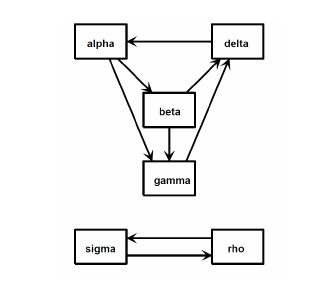
\includegraphics[width=0.5\textwidth]{images/anotherTinyWeb.png}
    \caption{Another Tiny Web}
    \label{fig:another-tiny-web}
\end{figure}

\subsubsection{What is the connectivity matrix G? Which are its entries?}

The connectivity matrix G is a mathematical representation which is used to describe the graph in the \ref{fig:another-tiny-web}. The matrix describes the connections between the nodes in a directed graph. For a directed graph with n nodes, the connectivity matrix G is an $ n \times n $ matrix, where the \(g_{ij}\) is defined as follows:

\begin{itemize}
    \item If there is a directed edge from node i to j then  $ g_{ij} = 1 $
    \item If there is no directed edge from node i to j then $ g_{ij} = 0 $
\end{itemize}

Bellow is the connectivity matrix G for the graph \ref{fig:connectivity-matrix}. In the graph there are 6 nodes and hence the connectivity matrix is a $ 6 \times 6 $ matrix. From the first row to the last row, and from first column to the last column, the nodes are ordered as \textit{alpa, beta, gamma, delta, rho, sigma}.

\begin{figure}[H]
    \centering
    \[ G =
        \begin{bmatrix}
            0 & 0 & 0 & 1 & 0 & 0 \\
            1 & 0 & 0 & 0 & 0 & 0 \\
            1 & 1 & 0 & 0 & 0 & 0 \\
            0 & 0 & 1 & 1 & 0 & 0 \\
            0 & 0 & 0 & 0 & 0 & 1 \\
            0 & 0 & 0 & 0 & 1 & 0 \\
        \end{bmatrix}
    \]
    \caption{Connectivity matrix G for the graph in \ref{fig:another-tiny-web}
        \label{fig:connectivity-matrix}}
\end{figure}






\subsubsection{What are the PageRanks if the hyperlink transition probability p assumes the default value of 0.85?}
In order to find the PageRanks for the graph in \ref{fig:another-tiny-web}, we first need to compute the variable G, U to use the function \textit{pagerank}. We know that \textit{p = 0.85}. The code for the same is shown bellow. \\

\begin{mcode}
    % Finding the PageRanks for the graph in \ref{fig:another-tiny-web}
    i = [1, 2, 3, 3, 4, 4, 5, 6] % row indices
    j = [4, 1, 1, 2, 2, 3, 6, 5] % column indices
    G = sparse(i, j, 1, 6, 6); % sparse matrix
    U = {"alpha", "beta", "gamma", "delta", "rho", "sigma"} % cell array 
    pagerank(U, G, 0.85) % PageRanks
\end{mcode}

Hence we have obtained the PageRanks for the graph in \ref{fig:another-tiny-web} as shown in Figure \ref{fig:pagerank-85}.\\

\begin{figure}[H]
    \centering
    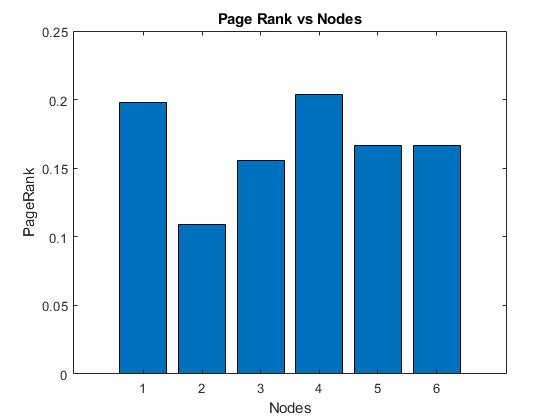
\includegraphics[width=0.5\textwidth]{images/pagerank-85.jpg}
    \caption{PageRank with p = 0.85}
    \label{fig:pagerank-85}
\end{figure}

As it can be seen from the Figure \ref{fig:pagerank-85}, the PageRank for the node \textit{delta} is the highest ranking amongst other nodes. The above data can also be visualzed in the form of a table in Figure \ref{tab:pagerank-table-85}.



\noindent
\begin{table}[H]
    \centering
    \begin{tabular}{|c|c|c|c|c|}
        \hline
        Index & Node  & PageRank & in & out \\
        \hline
        4     & delta & 0.2037   & 2  & 1   \\
        \hline
        1     & alpha & 0.1981   & 1  & 2   \\
        \hline
        5     & rho   & 0.1667   & 1  & 1   \\
        \hline
        6     & sigma & 0.1667   & 1  & 1   \\
        \hline
        3     & gamma & 0.1556   & 2  & 1   \\
        \hline
        2     & beta  & 0.1092   & 1  & 2   \\
        \hline
    \end{tabular}
    \caption{PageRank Table with p = 0.85}
    \label{tab:pagerank-table-85}
\end{table}


\subsubsection{Describe what happens with this example to both the definition of PageRank and the computation done by pagerank in the limit p → 1.}

\begin{figure}[H]
    \centering
    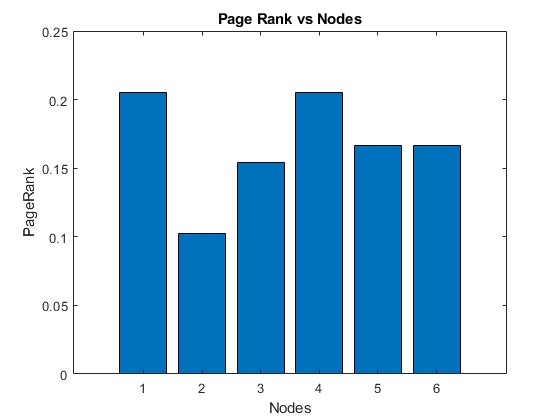
\includegraphics[width=0.5\textwidth]{images/pagerank-999.jpg}
    \caption{PageRank with p = 0.9999}
    \label{fig:pagerank-99}
\end{figure}

\noindent
\begin{table}[H]
    \centering
    \begin{tabular}{|c|c|c|c|c|}
        \hline
        Index & Node  & PageRank & in & out \\
        \hline
        4     & delta & 0.2051   & 2  & 1   \\
        \hline
        1     & alpha & 0.2051   & 1  & 2   \\
        \hline
        5     & rho   & 0.1667   & 1  & 1   \\
        \hline
        6     & sigma & 0.1667   & 1  & 1   \\
        \hline
        3     & gamma & 0.1556   & 2  & 1   \\
        \hline
        2     & beta  & 0.1092   & 1  & 2   \\
        \hline
    \end{tabular}
    \caption{PageRank Table with p = 0.9999}
    \label{tab:pagerank-table-85}
\end{table}



When the value of p is increased to close to 1, the PageRank of the nodes in the graph will more evenly distributed. This is because the probability of the random surfer to jump to another node is very low. This can be noticed in the Figure  as for the nodes with the same number of in and out links have the same PageRank. When p was set to 0.85 the weightage of the incoming links are much higher. However when it is set to 0.99999 it makes the PageRank of the nodes more evenly distributed. \\

\subsection{PageRanks by solving a sparse linear system [25 points]}

\subsubsection{Create pagerank1.m by modifying pagerank.m to use the power method instead of solving the sparse
    linear system.}

\begin{mcode}
    function x = pagerank1(U,G,p)
    %.....
    disp('Using Power Method Implementation\n');
    G = p * G * D;
    z = ((1 - p) * (c ~= 0) + (c == 0))/n;
    prec = 1e-16;
    x = e/n;
    x_old = zeros(size(x));

    while((norm(x - x_old)/ norm(x_old)) > prec)
    x_old = x;
    x = G * x + e * (z * x);
    disp(x - x_old)
    end
    %.....
    end
\end{mcode}

The apappropriate test for terminating the Power Method is with by getting the norm difference of x and x-old and seeing if it is bigger then the precision. The precision is set to $ 1e-16 $. If it is not bigger, then we assume that there has been a convergence and hence we terminate the Power Method. \\

\begin{table}[h]
    \centering


    \begin{tabular}{|c|c|c|c|c|}
        \hline
        index & page-rank & in  & out & url   \\
        $i$   & $x$       & $r$ & $c$ & $U$   \\
        \hline
        4     & 0.203694  & 2   & 1   & delta \\
        1     & 0.19814   & 1   & 2   & alpha \\
        5     & 0.166667  & 1   & 1   & rho   \\
        6     & 0.166667  & 1   & 1   & sigma \\
        3     & 0.155623  & 2   & 1   & gamma \\
        2     & 0.109209  & 1   & 2   & beta  \\
        \hline
    \end{tabular}
    \caption{PageRank1 table}
    \label{tab:pagerank}
\end{table}

The above example uses the six-node as an example to test the Power Method. The PageRank1 table is shown in Table \ref{tab:pagerank}. The pagerank1 function took in total \textbf{125} iterations to converge.

\subsubsection{\texorpdfstring{Create \texttt{pagerank2.m} by modifying \texttt{pagerank.m} to use the inverse iteration. Use your functions \texttt{pagerank1.m} and \texttt{pagerank2.m} (set $\alpha = 0.99$) to compute the PageRanks of the six-node example presented in Figure 1. Make sure you get the same result from each of your three functions.}{Create pagerank2.m by modifying pagerank.m to use the inverse iteration. Use your functions pagerank1.m and pagerank2.m (set α = 0.99) to compute the PageRanks of the six-node example presented in Figure 1. Make sure you get the same result from each of your three functions.}}

\begin{mcode}
    function x = pagerank1(U,G,p)
    %.....
    disp('Using Inverse Iteartion Implementation\n');
    G = p * G * D;

    z = ((1 - p) * (c ~= 0) + (c == 0))/n;
    A = p * G * D + e * z;

    prec = 1e-16;
    x = e/n;
    x_old = zeros(size(x));
    alpha = 0.99;
    iter = 0;
    while((norm(x - x_old)/ norm(x_old)) > prec)
        x_old = x;
        x = (alpha * I - A) \ x;
        x = x / norm(x,1);
        iter = iter + 1;
    end
    %.....
    end
\end{mcode}

\begin{figure}[H]
    \centering
    \begin{minipage}{0.45\textwidth}
        \centering
        \begin{tabular}{|c|c|c|c|c|}
            \hline
            index & page-rank & in  & out & url   \\
            $i$   & $x$       & $r$ & $c$ & $U$   \\
            \hline
            4     & 0.203694  & 2   & 1   & delta \\
            1     & 0.19814   & 1   & 2   & alpha \\
            5     & 0.166667  & 1   & 1   & rho   \\
            6     & 0.166667  & 1   & 1   & sigma \\
            3     & 0.155623  & 2   & 1   & gamma \\
            2     & 0.109209  & 1   & 2   & beta  \\
            \hline
        \end{tabular}
        \caption{PageRank1 table}
    \end{minipage}%
    \hfill
    \begin{minipage}{0.45\textwidth}
        \centering
        \begin{tabular}{|c|c|c|c|c|}
            \hline
            index & page-rank & in  & out & url   \\
            $i$   & $x$       & $r$ & $c$ & $U$   \\
            \hline
            4     & 0.203694  & 2   & 1   & delta \\
            1     & 0.19814   & 1   & 2   & alpha \\
            5     & 0.166667  & 1   & 1   & rho   \\
            6     & 0.166667  & 1   & 1   & sigma \\
            3     & 0.155623  & 2   & 1   & gamma \\
            2     & 0.109209  & 1   & 2   & beta  \\
            \hline
        \end{tabular}
        \caption{PageRank2 table}
    \end{minipage}
\end{figure}

While pagerank1 took \textbf{125} iterations to converge, pagerank2 took \textbf{52} iterations to converge.\\

\subsubsection{We now want to analyse the impact of alpha on the inverse iteration. Using the ETH500 example, set alpha equal to 0.8, 0.9, 0.95 and 1. Comment on the different number of iterations the four cases take until convergence. Analyse your results and explain what you observe.}




\noindent
\begin{table}[H]
    \centering
    \begin{tabular}{|c|c|c|}
        \hline
        Degree Centrality & Author    & Index \\
        \hline
        31                & Golub     & 1     \\
        \hline
        15                & Demmel    & 104   \\
        \hline
        13                & Plemmons  & 86    \\
        \hline
        12                & Schreiber & 44    \\
        \hline
        12                & Heath     & 81    \\
        \hline
    \end{tabular}
    \caption{Top 5 authors with highest degree centrality}
\end{table}

As it can be sene from the table above, as the value of $\alpha$ increases the number of iterations required to converge also increases the iteration as well increases with it. This is because as the value of $\alpha$ increases the value of $ \frac{1}{\lambda_1 - \alpha} $ decreases. Hence the convergence is slower. \\

\subsubsection{Use your functions pagerank1.m and pagerank2.m (set alpha = 0.99) to compute the PageRanks of three selected graphs (web1.mat, web2.mat and web3.mat). Report on the convergence of the two methods
for these subgraphs and summarize the advantages and disadvantages of the power method implemented in
pagerank1.m against the inverse iteration in pagerank2.m.}
\begin{figure}[H]
    \centering
    \begin{tabular}{|c|c|c|}
        \hline
        Website & PageRank 1 Itearation & PageRank 2 Iteration \\
        \hline
        Web 1 & 173 & 98 \\
        Web 2 & 145 & 74 \\
        Web 3 & 212 & 93 \\
        \hline
    \end{tabular}
    \caption{PageRank1 vs PageRank2}
\end{figure}

From the above data which was computed it can be seen that PageRank2 perfomed better in terms of iteration as compare to PageRank1. However PageRank1 which uses the Power Method is computationly cheaper than PageRank2 which uses the Inverse Iteration. Due to this the time it takes to compute PageRank1 is much less as compare to PageRank2. Hence PageRank1 is usefull in majority of the cases, but takes much more iterations to converge. In the other PageRank1 congerges in less iterations, but is very senstive to its alpha value. \\

\subsection{The Reverse Cuthill--McKee Ordering [5 points]}

\begin{figure}[H]
    \centering
    \begin{minipage}[b]{0.45\textwidth}
        \centering
        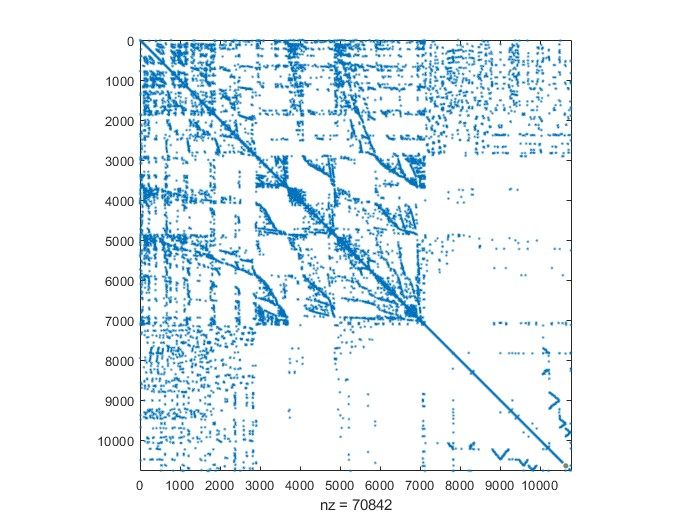
\includegraphics[width=\textwidth]{images/exc5.jpg}
        \caption{Original Matrix}
    \end{minipage}
    \hfill
    \begin{minipage}[b]{0.45\textwidth}
        \centering
        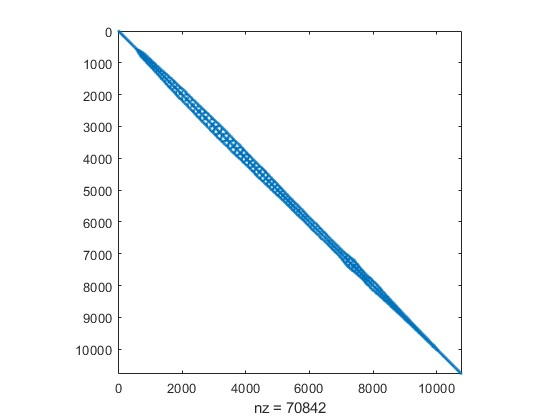
\includegraphics[width=\textwidth]{images/exc5n.jpg}
        \caption{Reverse Cuthill McKee Matrix}
    \end{minipage}
\end{figure}


\begin{figure}[H]
    \centering
    \begin{minipage}[b]{0.45\textwidth}
        \centering
        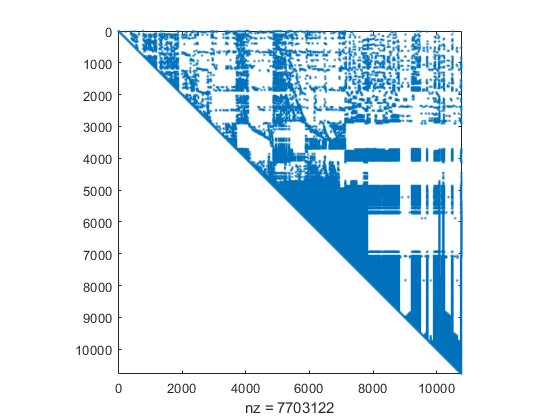
\includegraphics[width=\textwidth]{images/exc5o.jpg}
        \caption{Cholesky factorization of the original matrix}
    \end{minipage}
    \hfill
    \begin{minipage}[b]{0.45\textwidth}
        \centering
        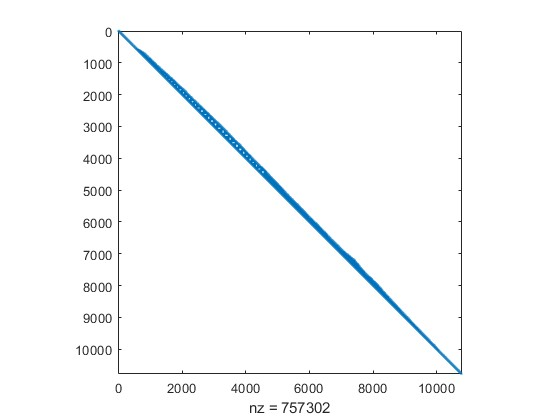
\includegraphics[width=\textwidth]{images/s.jpg}
        \caption{Cholesky factorization of the reverse Cuthill McKee matrix}
    \end{minipage}
\end{figure}

The non-zero elemnts in the Cholesky Factorization of the original matrix is \textbf{7703122}, while for the Cholesky Factorization of the reverse Cuthill McKee matrix is \textbf{757302}.
\subsection{Sparse Matrix Factorization [10 points]}
\subsubsection{Construct matrix A for the case n = 10 and explicitly write down its entries. How many non-zero elements does it have?}
\[ A =
    \begin{bmatrix}
        10 & 1  & 1  & 1  & 1  & 1  & 1  & 1  & 1  & 1  \\
        1  & 11 & 0  & 0  & 0  & 0  & 0  & 0  & 0  & 1  \\
        1  & 0  & 12 & 0  & 0  & 0  & 0  & 0  & 0  & 1  \\
        1  & 0  & 0  & 13 & 0  & 0  & 0  & 0  & 0  & 1  \\
        1  & 0  & 0  & 0  & 14 & 0  & 0  & 0  & 0  & 1  \\
        1  & 0  & 0  & 0  & 0  & 15 & 0  & 0  & 0  & 1  \\
        1  & 0  & 0  & 0  & 0  & 0  & 16 & 0  & 0  & 1  \\
        1  & 0  & 0  & 0  & 0  & 0  & 0  & 17 & 0  & 1  \\
        1  & 0  & 0  & 0  & 0  & 0  & 0  & 0  & 18 & 1  \\
        1  & 1  & 1  & 1  & 1  & 1  & 1  & 1  & 1  & 19 \\
    \end{bmatrix}
\]

The total number of non-zero elements are \textbf{44}.

\subsubsection{We now want to derive a general formula to compute the number of non-zero entries. Show that, for a given matrix \texorpdfstring{\(A \in \mathbb{R}^{n \times n}\)}{A in R^n x n} with this structure, the number of non-zero elements is \(5n - 6\).}

In order to dervive a general formula to compute the number of non-zero entries in the matrix we should first observe the matrix and see some of its properties. We can observie that the matrix boundries and its diagonal are all non-zero. This is a really important property as wel can use this to derive the general formula. \\

We can see that there is 2 rows (top-most and bottom-most) which are non-zero, there are 2 columns (left-most and right-most) and at last there is a diagnol matrix. We can see the size of there is n, in this case 10. Hence we can dervive that the number of non-zero elements are $(2 + 2 + 1)n = 5n$. However as it can be noticed we are couting some of the non-zero elements more than once. Hence we need to subtract the number of non-zero elements which are counted more than once. \\

Finding all the elements being counted more than once:

\begin{itemize}
    \item $A_{11}$ is being counted 2 extra times.
    \item $A_{nn}$ is being counted 2 extra times.
    \item $A_{1n}$ is being counted 1 extra time.
    \item $A_{n1}$ is being counted 1 extra time.
\end{itemize}

Hence in total there are 6 elements which are being counted more than once. Hence the total number of non-zero elements are: $$5n - 6$$.

\subsubsection{Write a function A construct(), which takes as input n and returns, as output, the matrix A defined in Eq. 14 and its number of non-zero elements nz. Test your function in a script ex2c.m for n = 10 and compare your results with those you obtained in 6.1. Furthermore, within the same script, visualise the non-zero structure of matrix A by using the command spy().}

\begin{mcode}
    function [A,nz] = A_construct(n)
    A = zeros(n);       % initialize matrix
    for i = 1:n         % iterate over rows
    for j = 1:n     % iterate over columns
    if i == j
    A(i, j) = n + i - 1;
    elseif i == 1 || i == n || j == 1 || j == n
    A(i, j) = 1;
    else
    A(i, j) = 0;
    end
    end
    end
    nz = nnz(A);
    end
\end{mcode}

By running the above function, which replicates the Eq. 14, we obtained the same matrix which we had obtained in 6.1. The number of non-zero elements are also the same. The spy plot for the matrix A is shown in Figure \ref{fig:spy-plot}.

\begin{figure}[H]
    \centering
    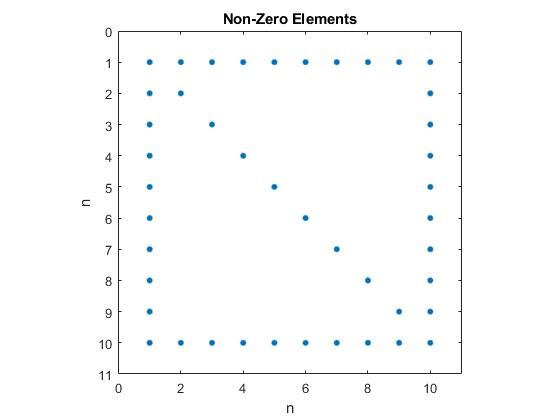
\includegraphics[width=0.5\textwidth]{images/nbyn.jpg}
    \caption{Spy plot for the matrix A}
    \label{fig:spy-plot}
\end{figure}

\subsubsection{Using again the spy() command, visualize side by side the original matrix A and the result of the Cholesky factorization (chol() in Matlab).}

\begin{figure}[H]
    \centering
    \begin{minipage}[b]{0.45\textwidth}
        \centering
        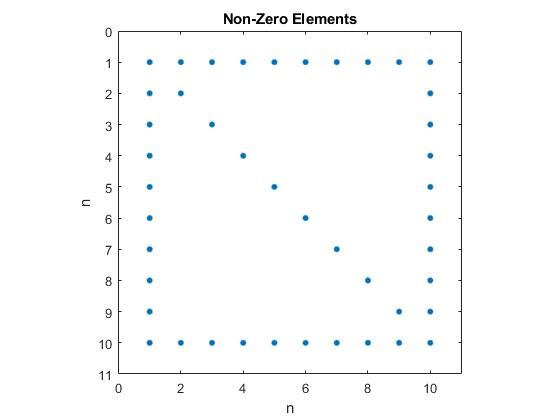
\includegraphics[width=\textwidth]{images/nbyn.jpg}
    \end{minipage}
    \hfill
    \begin{minipage}[b]{0.45\textwidth}
        \centering
        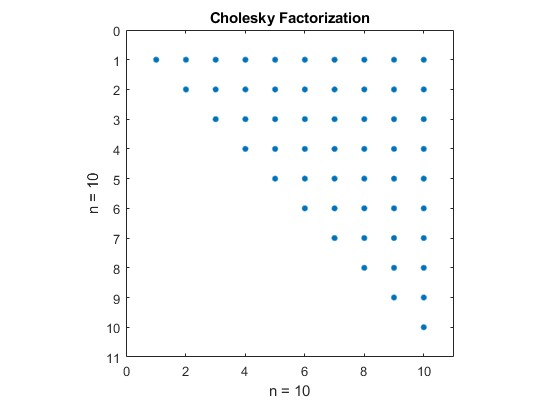
\includegraphics[width=\textwidth]{images/chol.jpg}
    \end{minipage}
    \caption{Spy plot for the matrix A vs Cholesky factorization for the matrix A}
    \label{fig:comparison}
\end{figure}

\subsubsection{Explain why, for n = 100, 000, using chol() to solve Ax = b for a given right-hand-side vector b would be problematic. Are there ways to mitigate this issue?}

When n = 100,000 is run using chol() Matlab gives an error saying there is not enough memory for the operation to take place. This is because the matrix A is a dense matrix and hence it takes a lot of memory to perform all the computing with chol(). The complexity for this operation is $O(n^3)$. Hence if this operations is needed to perform either a powerfull machine is required or the matrix A needs to formed as a lower triangular matrix which would make the computation much faster. \\

\subsection{Degree Centrality [5 points]}
\noindent
\begin{table}[H]
    \centering
    \begin{tabular}{|c|c|c|}
        \hline
        Degree Centrality & Author    & Index \\
        \hline
        31                & Golub     & 1     \\
        \hline
        15                & Demmel    & 104   \\
        \hline
        13                & Plemmons  & 86    \\
        \hline
        12                & Schreiber & 44    \\
        \hline
        12                & Heath     & 81    \\
        \hline
    \end{tabular}
    \caption{Top 5 authors with highest degree centrality}
\end{table}

The above table repersents the Top 5 authors with the highest degree centrality. The degree centrality is the number of edges that are connected to the node. In this case the node is the author. Hence the degree centrality is the number of coauthors that the author has. \\

\subsection{The Connectivity of the Coauthors [5 points]}

\begin{figure}[H]
    \centering
    \begin{tabular}{|l|l|}
        \hline
        Authors & Common Authors \\
        \hline
        Golub, Moler & Wilkinson, VanLoan \\
        Golub, Saunders & Saunders \\
        TChan, Demmel & Schreiber, Arioli, Duff, Heath \\
        \hline
    \end{tabular}
    \caption{Table of Common Authors}
\end{figure}

\subsection{PageRank of the Coauthor Graph [5 points]}

\begin{figure}[H]
    \centering
    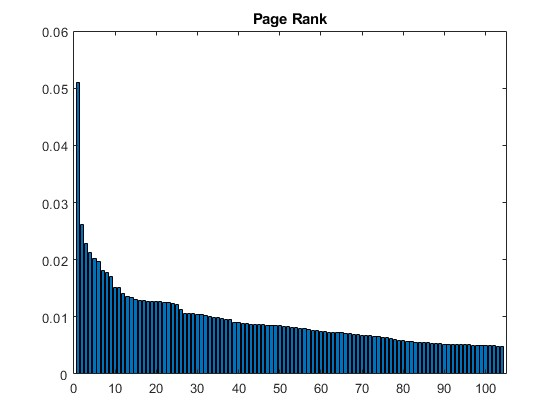
\includegraphics[width=0.5\textwidth]{images/exc9.jpg}
    \caption{PageRank of all the Authors}
    \label{fig:exc9}
\end{figure}

In the Figure \ref{fig:exc9} the PageRank of all the authors is shown. The PageRank1 was modified which used the power method, in which it took the authors as the inputs to compute the pagerank for them. This script can be found as named as \textit{exc9.m}. \\

\end{document}
